\section{Análise teórica do passa-baixas}
  Como apresentado previamente, os filtros passa-baixas tem como característica a capacidade de atenuar sinais com frequências grandes, acima de uma frequência linear de corte, $f_c$ ou frequência angular de corte, $\omega_c$, definidas. Uma topologia indicada para se utilizar é a de um circuito RC de resistor em série com um capacitor em que a saída de tensão do circuito ocorre sobre o capacitor.

  Considerando o circuito RC série com a saída sobre o capacitor, $v_{out}$, dado na figura \ref{fig:esquematico_passa_baixas}, em regime permanente senoidal (RPS), alimentado por um gerador ideal senoidal, $v_{in}$.

  \begin{figure}[H]
    \centering
    \caption{Esquemático de um circuito passa-baixas}
    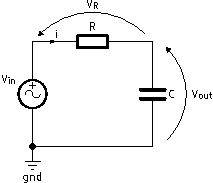
\includegraphics[width = 0.6 \linewidth]{passa-baixas.pdf}
    \fontfigure{Elaboração Própria (Kicad)(\the\year)}
    \label{fig:esquematico_passa_baixas}
  \end{figure}

  É possível obter as equações e os gráficos do módulo e fase da resposta em frequência do circuito considerando a impedância dos componentes como $R$ e $\frac{1}{j \omega C}$, resistor e capacitor, respectivamente, as tensões dadas em fasores como $\hat{v}_{in}$, $\hat{v}_{R}$ e $\hat{v}_{out}"$, sendo as tensões sobre a fonte, o resistor e o capacitor, respectivamente e a corrente do circuito dada como $\hat{i}$.

  Utilizando as relações constitutivas dos bipolos dados temos que:

  \begin{equation*}
    \begin{cases}
      \hat{v}_{out} = \frac{1}{j \omega C} \cdot \hat{i} \\
      \hat{v}_{R} = R \cdot \hat{i}
    \end{cases}
  \end{equation*}

  Pela segunda lei de Kirchhoff (\textit{Kirchhoff's Voltage Law}), tem-se:

  \begin{equation} 
    \mathbf{KVL:} \quad \hat{v}_{in} = \hat{v}_{R} + \hat{v}_{out} = R \cdot \hat{i} + \hat{v}_{out}
    \label{eq:kvl_passa_baixas}
  \end{equation}

  Analisando o circuito, considerando-o com apenas um bipolo de impedância total $Z$, pode-se obter a corrente do circuito isolando-a na equação:

  \begin{equation}
    \hat{v}_{in} = Z \cdot \hat{i} = \left( R + \frac{1}{j \omega C} \right) \cdot \hat{i} \Rightarrow \hat{i} = \frac{\hat{v}_{in}}{R + \frac{1}{j \omega C}}
    \label{eq:corrente_passa_baixas}
  \end{equation}

  Com isso, substituindo a equação \ref{eq:corrente_passa_baixas} na \ref{eq:kvl_passa_baixas} é possível obter a expressão da resposta em frequência dada por $G(j \omega)$.

  \begin{equation*}
    \sp{(\ref{eq:corrente_passa_baixas}) \rightarrow (\ref{eq:kvl_passa_baixas})}
    \quad \hat{v}_{in} = R \cdot \frac{\hat{v}_{in}}{R + \frac{1}{j \omega C}} + \hat{v}_{out} \Rightarrow \frac{\hat{v}_{out}}{\hat{v}_{in}} = 1 - \frac{R}{R + \frac{1}{j \omega C}} = \frac{1}{1 + j \omega R C} = G(j \omega) 
  \end{equation*}

  \begin{equation}
    \therefore \quad G(j \omega) = \frac{1}{\sqrt{1 + \left(\omega R C\right)^2}} \phase{-\arctan(\omega R C)}
    \label{eq:ganho_passa_baixas}
  \end{equation}

  A partir da expressão, \ref{eq:ganho_passa_baixas}, obtida é possível construir os gráficos, apresentados na figura \ref{fig:grafico_passa_baixas}, que apresentam o valor em módulo e da fase de $G(j\omega)$ em função da frequência angular, $\omega$, analisando os gráficos é possível reconhecer e calcular pontos importantes da curva, como os pontos para que $|G(j0)| = 1$ para $\omega = 0$, que $ \lim_{\omega\to\infty} |G(j\omega)| = 0$ e $|G(j \omega)| = \frac{1}{\sqrt{2}}$, para $\omega = \frac{1}{RC}$, que indica o momento em que a potência média de saída cai pela metade de seu valor máximo, sendo o momento onde ocorre a frequência de corte, logo $\omega_c = \frac{1}{RC}$.

  \begin{figure}[H]
    \centering
    \caption{Gráficos do circuito passa-baixas, módulo e fase, respectivamente}
    \begin{subfigure}{0.5 \linewidth}
      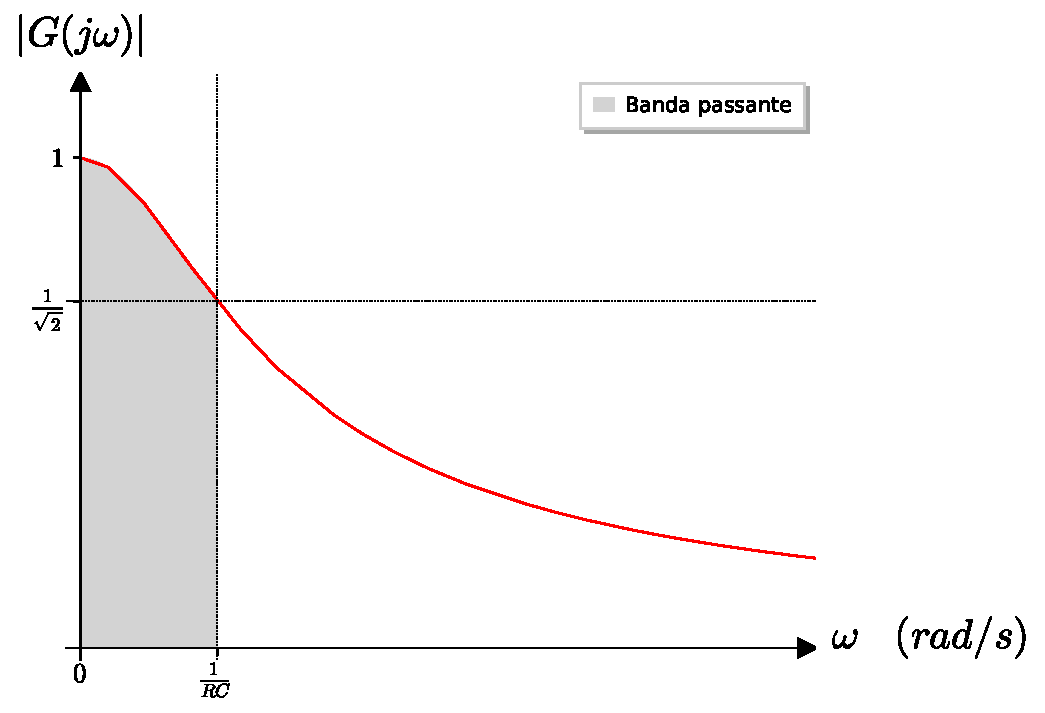
\includegraphics[width = \linewidth]{plot-0.pdf}
    \end{subfigure}%
    \begin{subfigure}{0.5 \linewidth}
      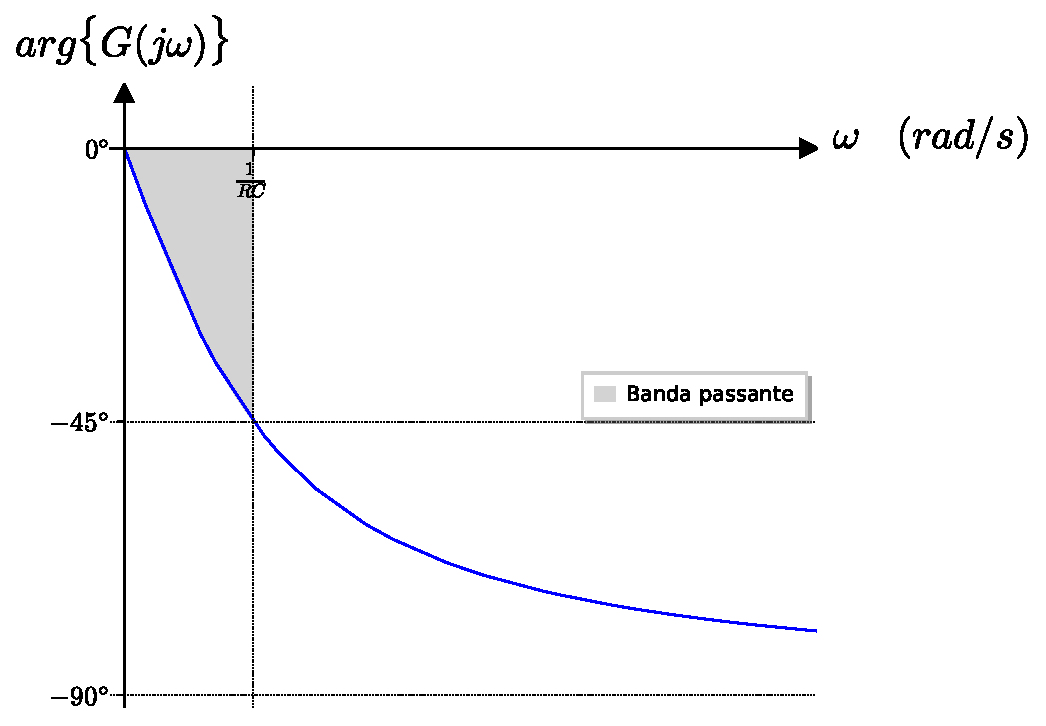
\includegraphics[width = \linewidth]{plot-1.pdf}
    \end{subfigure}
    \fontfigure{Elaboração Própria (\the\year)}
    \label{fig:grafico_passa_baixas}
  \end{figure}

  Outras características obtidas analisando o gráfico é que de fato ele se comporta como um filtro passa-baixas, já que o módulo da razão da tensão de saída pela de entrada, diminui drasticamente conforme se aumenta a frequência angular, em torno da frequência de corte.
  